\section{Framework}

In this section, we introduce the details of how to represent source code and how to use the representation vector of source code to generate comments.

\begin{figure*}[th]
\begin{minipage}{0.15\linewidth}
  \begin{lstlisting}

  if (!found){
    allFound = false;
  }
  if (allFound){
    return true;
  }
\end{lstlisting}
 \centerline{source code}
\end{minipage}
\hfill
\begin{minipage}{0.9\linewidth}
  \centering
	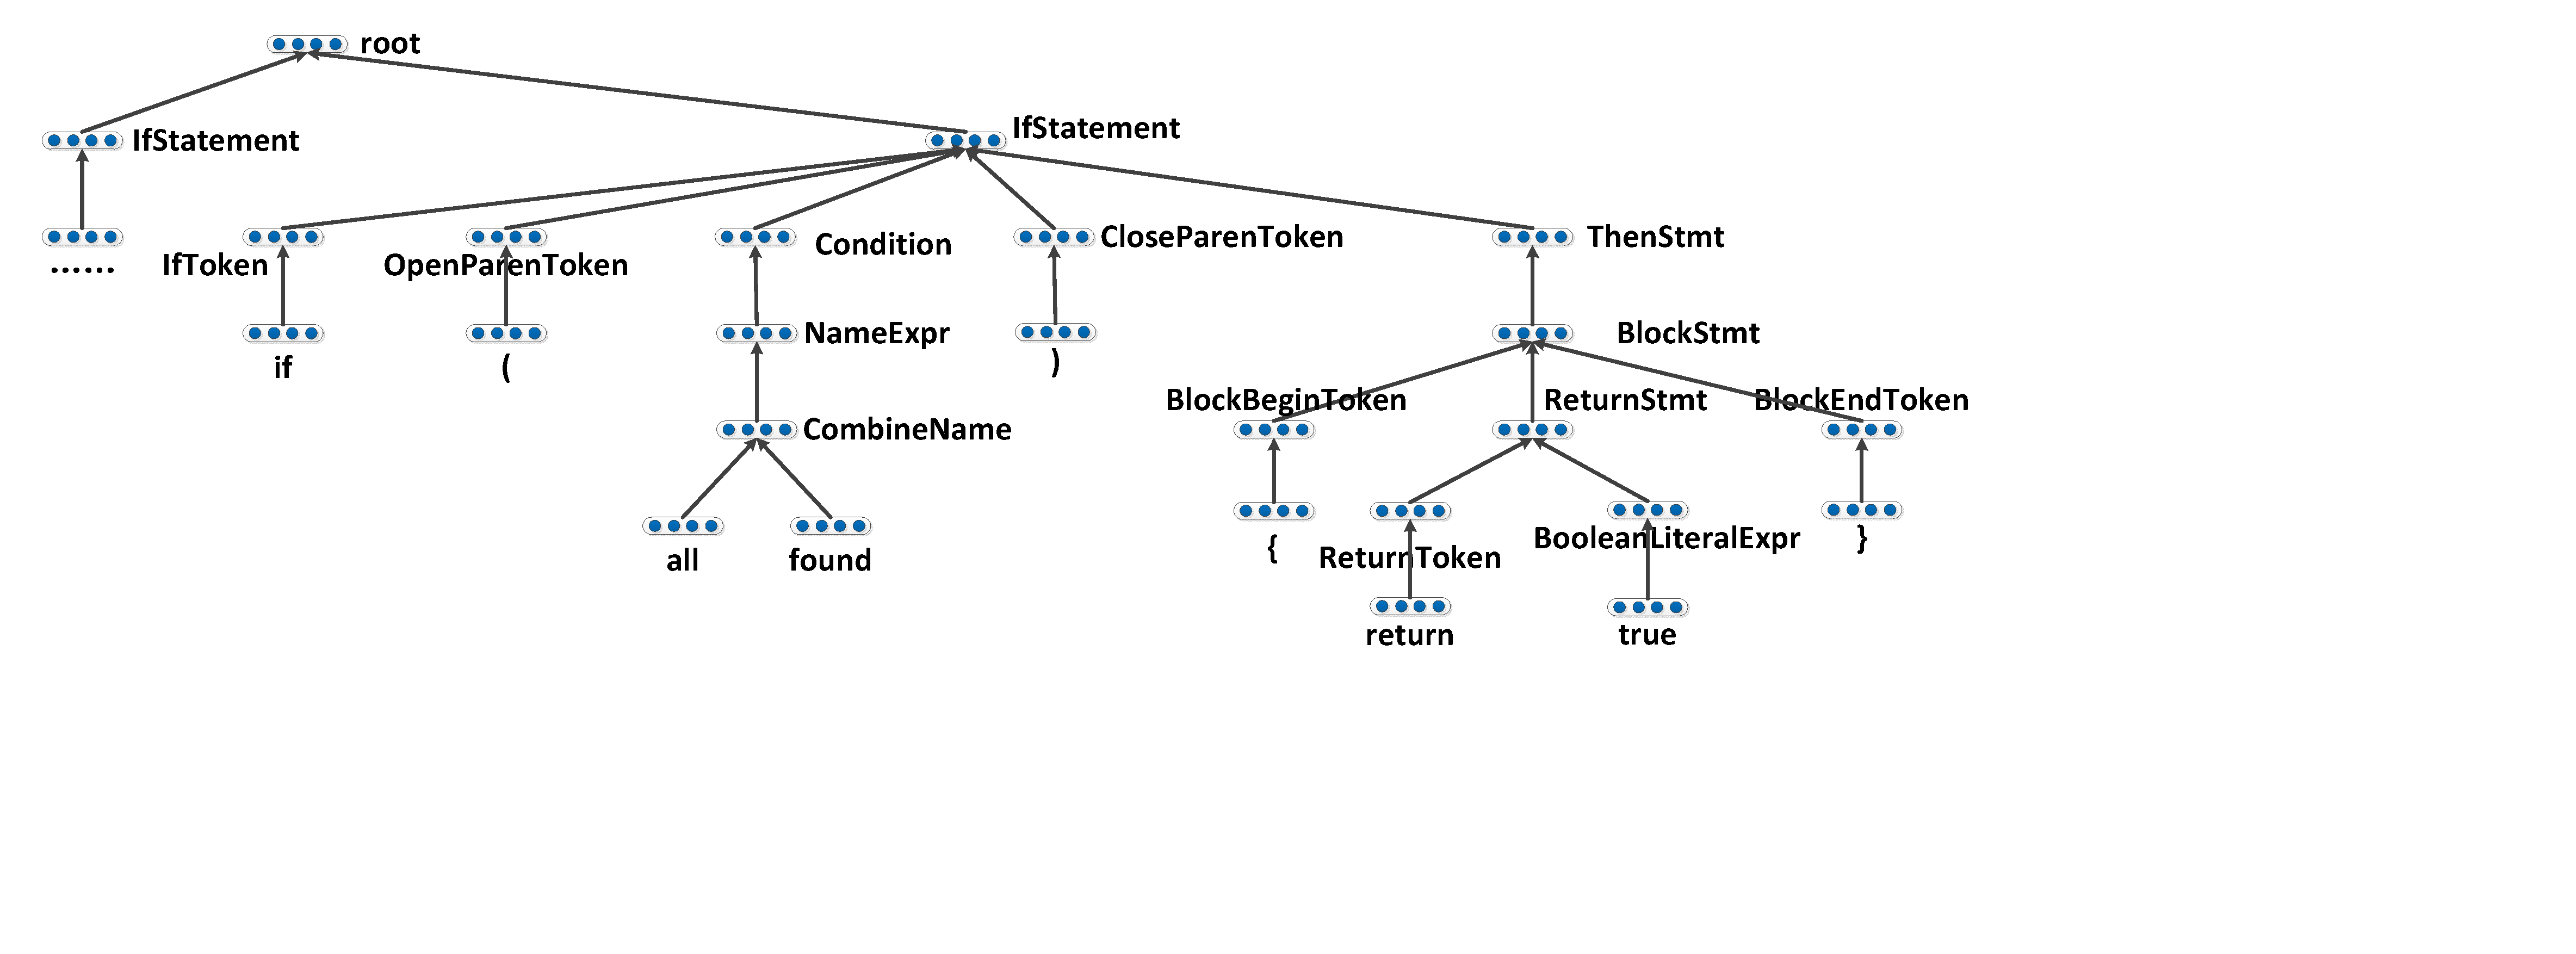
\includegraphics[width=0.9\linewidth]{img/tree_rnn.pdf}
 \centerline{Code-RNN}
\end{minipage}

\caption{Code-RNN Example}\label{fig:code_rnn}
\end{figure*}


\subsection{Code Representation}

We propose a new kind of recursive neural network called Code-RNN to encapsulate
the critical structural information of the source code.
Code-RNN is an arbitrary tree form while other recursive neural nets
used in NLP are typically binary trees. Fig. \ref{fig:code_rnn} shows an
example of Code-RNN for a small piece of Java code.

In Code-RNN, every parse tree of a program is encoded into a neural network,
where the structure of the network is exactly the parse tree itself and
each syntactic node in the
parse tree is represented by a vector representation.~\footnote{We use
JavaParser from \url{https://github.com/javaparser/javaparser} to
generate parse tree for Java code in this paper.}
%We add the root node in the parse tree first, then the statements
%as the children of root node. In Fig. \ref{fig:code_rnn}, we can see the code snippet has two if statement, so the root node has two same children. We only show the detail of the second if statement and the ``......' represents all nodes of the first if statement. For the if statement, it has the three children statements, ``Condition'',``ThenStmt'' and ``ElseStmt''. In this example, it don't have the children ``ElseStmt'' so we don't put it in the parse tree. Then we can construct our parse tree recursively.
One unique internal node ``CombineName'' indicates a compound identifier that is
the concatenation of several primitive words, for example, ``allFound'' can be split into
``all'' and ``found''. More on the semantics of identifier will be discussed later in
this section.

%Besides the vector representation $V_{c}$ for each node in the tree, parameters $W$ and bias $b$, these three kinds of parameter are tuned during training process.

There are two models for the Code-RNN, namely \emph{Sum Model} and \emph{Average Model}:
%\KZ{Why not another model that preserves order of the children of any given node?}
\begin{enumerate}
\item{Sum Model}
\begin{equation}\label{eq:code_rnn_sum}
V = V_{node} + f(\textbf{W} \times \sum_{c \in C}{ V_{c}} + \textbf{b})
\end{equation}

\item{Average Model}
\begin{equation}\label{eq:code_rnn_average}
V = V_{node} + f(\textbf{W} \times \frac{1}{n}\sum_{c \in C}{V_{c}} + \textbf{b})
\end{equation}
\end{enumerate}
Here $V$ is the vector representation of sub-tree rooted at $N$;
$V_{node}$ is the vector that represents the syntactic type of $N$ itself, e.g.,
{\em IfStatement};
$C$ is the set of all child nodes of $N$; $V_{c}$ is the vector that represents
a subtree rooted at $c$, one of $N$'s children.
During the training, $W$ and $b$ are tuned.
$V$, $V_{node}$ and $V_{c}$ are calculated based on the structure
of neural network. $f$ is \emph{RELU} activation function.


%$V$ is the new representation vector, $V_{node}$ is the unique vector for every node type, $n$ is the number of children nodes, $c$ is the index of children node type, and $C$ is the index set.
%$\textbf{W}$ is the weight matrix and $\textbf{b}$ is the bias and
%all nodes are the same. $f$ is \textbf{RELU} activation function. \KZ{Rephrase the above. Not clear! What is $V_{node}$? What is
%$V$?}

These equations are applied recursively, bottom-up through the Code-RNN at
every internal node, to obtain the vector representation of the root node,
which is also the vector of the entire code piece.

\subsubsection{Identifier Semantics}
\label{sec:identifier}
%\KZ{\textcolor{red}{This section needs to be expanded significantly. I still don't understand
%Table \ref{table:abbr}. If you use rules, you should explicitly say what those
%rules are to recover the original words from the abbreviations. If you use
%some algorithm, better include the listing of the pseudo-code.}}


In this work, we adopt two ways to extract the semantics from the identifiers.
One is to split all the long forms to multiple words and
the other one is to recover the full words from abbreviations.

Table \ref{table:splitID} shows some example identifiers and the results
of splitting. Many identifiers in the source code are combination of English words,
with the first letter of the word in upper case, or joined together using
underscores. We thus define simple rules to extract the original
English words accordingly. These words are further connected by the
``CombineName'' node in the code-RNN.
%For example, we can split the expression ``DoubleMatrix(confusionMatrix)''
%into two lists. The first list contains ``double'' and ``matrix'',
%and the second contains ``confusion'' and ``matrix''.

Table \ref{table:abbr} shows some abbreviations and
their intended meaning. We can infer the full-versions by
looking for longer forms in the context of the identifier in the code.
Specifically, we compare the identifier with the word list generated from
the context of the identifier to see whether the identifier's name
is a substring of some word from the list, or is the combination of
the initial of the words in the list.
If the list contains only one word, we just check if the identifier
is part of that word. If so, we conclude that the identifier is the
abbreviation of that word with higher probability.
If the list contains multiple words, we can collect all the initials 
of the words in the list to see whether the identifier is part of
this collection. Suppose the code fragment is
\begin{lstlisting}
Matrix dm = new DoubleMatrix(confusionMatrix);
\end{lstlisting}
%After this process we can get most of the full names of the parameters.
We search for the original words of ``dm'' as follows.
Since ``dm'' is not the substring of any word in the context,
we collect the initials of the contextual words in a list:
``m'' ``dm'' and ``cm''.
Therefore, ``dm'' is an abbreviation of ``DoubleMatrix''.

\begin{table}[th]
\caption{\label{table:splitID} Example of Split Identifiers}
\center
\scriptsize{
\begin{tabular}{|c|c|}
\hline
Identifier & Words \\
\hline \hline
contextInitialize & context, initialize\\
\hline
apiSettings & api, settings\\
\hline
buildDataDictionary & build, data, dictionary\\
\hline
add\_result & add, result\\
\hline
\end{tabular}
}
\end{table}

\begin{table}[th]
\caption{Example of Abbreviation}
\label{table:abbr}
\center
\scriptsize{
\begin{tabular}{|c|c|c|}
\hline
Abbreviation & Origin & Context\\
\hline \hline
val & value & key.value()\\
\hline
cm & confusion, matrix & new ConfusionMatrix()\\
\hline
conf & configuration & context.getConfiguration()\\
\hline
rnd & random & RandomUtils.getRandom()\\
\hline
\end{tabular}
}
\end{table}

\subsubsection{Training}
Each source code block in the training data has a class label.
Our objective function is:
\begin{equation}
\small{
\mathop{\arg\min} CrossEntropy(softmax(W_{s}V_{m} + b_{s}),V_{label})\label{eq:object}
}
\end{equation}
where $V_{m}$ is the representation vector of source code, $V_{label}$ is
an one-hot vector to represent the class label.
$W_{s}$ and $b_{s}$ are parameters for softmax function and will be
tuned during training.  We use AdaGrad~\cite{duchi2011adaptive} to apply
unique learning rate to each parameter.

%When we train the Code-RNN, we begin from all leaf nodes.
%We use the node ``CombineName'' in Fig. \ref{fig:code_rnn} as an example.
%Now we totally have three vectors $V_{all}$, $V_{found}$ and $V_{CombineName}$ with respect to node ``all'', ``found'' and ``CombineName''. For node ``CombineName'', it has two children ``all'' and ``found'', so the vector representation $V_{train\_CombineName}$ of node ``CombienName'' during training will be calculated as $V_{CombineName} + f(W \times (V_{all} + V_{found}) + b)$ in Sum Model or $V_{CombineName} + f(W \times 0.5 \times (V_{all} + V_{found}) + b)$ in Average Model. Then we can get the vector representation $V_{train\_NameExpr}$ of the parent of node ``CombineName'', ''NameExpr'', during training. Recursively, we can get the vector of node ``root'' as $V_{train\_root}$, and we regard $V_{train\_root}$ as the vector representation of the whole method.
%
%For classification problem, we apply $softmax$ function to $V_{train\_root}$ to train. During back-propagation process, we through the whole network from root node to all leaf nodes recursively and tune all parameters in Equation \ref{eq:code_rnn_sum} and Equation \ref{eq:code_rnn_average} except $n$ to approach to the best situation.

%\subsubsection{Test}
%
%No matter what problem we want to solve, we can use our Code-RNN model to get a meaningful vector representation of methods or parse trees, just repeat the forward-propagation of training time and get the vector representation of root node $V_{train\_root}$. Then we can use this vector to do following works such as classification problem and comment generation. More details will be discussed later.
%


\subsection{Comment Generation}
%A. Karpathy and L. Fei-Fei~\cite{karpathy2015deep} proposed a meaningful method to generate image descriptions. In their model, they connect CNN and RNN(Recurrent Neural Network) end-to-end to generate description. This is different from other language model based on Recurrent Neural Network \cite{elman1990finding,sutskever2011generating,mikolov2010recurrent}, they generate sentences by defining a probability distribution of the next word in a sequence given the current word and context from previous time steps. We also use this model but replace CNN to our model Code-RNN, and feed Code-RNN vector in every step of RNN(Recurrent Neural Network).
Existing work~\cite{elman1990finding,sutskever2011generating,mikolov2010recurrent} has used Recurrent Neural Network to generate sentences.
However, one challenge to utilize the code block representation vector
in Recurrent NN is that we can not feed the code block representation vector to
the Recurrent NN cell directly.
%\KZ{What is the difficulty here?}.
We thus propose a variation of the GRU based RNN.
Fig. \ref{fig:comment_generate} shows our comment generation process.

\begin{figure}[th]
\centering
	\includegraphics[width=0.8\linewidth]{img/comment_generation.pdf}
\caption{Comment Generation}\label{fig:comment_generate}
\end{figure}


We use pre-trained model Code-RNN to get the representation vector of
the input code block $V_{m}$. This vector $V_{m}$ is fixed during training of
comment generation model. Then we feed code block vector into the
RNN (Recurrent Neural Network) model at every step.
For example in Fig.~\ref{fig:comment_generate}, we input the START token
as the initial input of model and feed the code block vector into the hidden
layer. After calculating the output of this step, we do the
back-propagation. Then at step two, we input the word ``gets'' and
feed the code block vector $V_{m}$ into hidden layer again,
%this is different from A. Karpathy and L. Fei-Fei~\cite{karpathy2015deep},
and receive the $h_{t-1}$ from the step one. We repeat the above
process to tune all parameters. The equations of comment generation model
are listed below.

\begin{align}
z_{t} &= \sigma(W_{z}\cdot[h_{t-1},x_{t}])\\
r_{t} &= \sigma(W_{r}\cdot[h_{t-1},x_{t}])\\
c_{t} &= \sigma(W_{c}\cdot[h_{t-1},x_{t}]) \label{eq:ct} \\
\tilde{h_{t}} &= tanh(W\cdot[r_{t}*h_{t-1},c_{t}*V_{m},x_{t}]) \label{eq:ct2}\\
h_{t} &= (1-z_{t})*h_{t-1} + z_{t}*\tilde{h_{t}} \\
y_{t} &= softmax(W_{oh}h_{t} + b_{o})
\end{align}
where $V_{m}$ is the code block representation vector, $h_{t-1}$ is the previous state and $x_{t}$ is the input word of this step.

To better use the code block vectors, our model differs from existing RNNs,
particularly in the definition of $c_{t}$ in the Equation \ref{eq:ct}
and \ref{eq:ct2}.
The new RNN cell, illustrated in Fig. \ref{fig:new_gru},
aims to strengthen the effect of code block vectors.
This modified GRU is hereinafter called \emph{Code-GRU}.
Code block vector contains all information of code block but not all information
is useful at all steps. Therefore, we add a new gate called choose gate
to determine which dimension of code block vector would work in Code-GRU.
In Fig \ref{fig:new_gru}, the left gate is the choose gate,
and the other two gates are the same as the original GRU.

\begin{figure}[th]
\centering
	\includegraphics[width=0.8\linewidth]{img/NewGRU.pdf}
\caption{Structure of Code-GRU}\label{fig:new_gru}
\end{figure}

%The equation of \textbf{GODE-GRU}:
%\begin{align}
%z_{t} &= \sigma(W_{z}\cdot[h_{t-1},x_{t}])\\
%r_{t} &= \sigma(W_{r}\cdot[h_{t-1},x_{t}])\\
%c_{t} &= \sigma(W_{c}\cdot[h_{t-1},x_{t}])\\
%\tilde{h_{t}} &= tanh(W\cdot[r_{t}*h_{t-1},c_{t}*V_{m},x])\\
%h_{t} &= (1-z_{t})*h_{t-1} + z_{t}*\tilde{h_{t}}
%\end{align}


During test time, we input the ``START'' token at first and choose the 
most probable word as the output. Then from the second step the input words of every step are the output words of previous one step until the output is ``END'' token. So that we can get an automatically generated comment for code blocks 
in our model.

To gain better results, we also apply the beam search while testing.
We adopt a variant of beam search with a length penalty described
in~\cite{wu2016google}. In this beam search model, there are two parameters:
beam size and weight for the length penalty. We tune these
two parameters on the validation set to determine which values to use.
Our tuning ranges are:
\begin{itemize}
    \item beam size: [1, 2, 3, 4, 5, 6, 7, 8, 9, 10]
    \item weight for the length penalty: [0, 0.1, 0.2, 0.3, 0.4, 0.5, 0.6, 0.7, 0.8, 0.9, 1.0]
\end{itemize}

